\documentclass[a4paper,11pt]{article}

% Add style file.
\usepackage{explanation}

% TMP...
\usepackage{lipsum}

% Add bib file for literature.
\addbibresource{explanation.bib}

\title{Implementing Deep Visual Odometry\\{\large Final Task of the course \emph{Implementing ANNs with Tensorflow}}}
\author{Rasmus Diederichsen \and Christian Heiden \and Alexander Mock\\\and \href{mailto:rdiederichse@uos.de}{rdiederichse@uos.de}\and \href{mailto:cheiden@uos.de}{cheiden@uos.de} \and \href{mailto:amock@uos.de}{amock@uos.de}}

\begin{document}

% Title
\maketitle


% --------------------- %
% SECTION: INTRODUCTION %
% --------------------- %
\section{Introduction}
\label{sec:introduction}
% TODO: Explain how visual odometry is useful
% TODO: Explain the structure of this paper
In robotics, the localization of a robot within its environment is an essential task. Especially in the days of autonomously driving vehicles this field of research receives a significant amount of attention. There are many ways to perform robot localization and usually several methods are used at the same time in order to improve reliability of the whole system. The main task of a localization algorithm is to repeatedly estimate the current pose of the robot. A pose is a 6-\emph{d} vector containing the $x$, $y$, $z$ positional values, as well as the \emph{yaw}, \emph{pitch}, and \emph{roll} values representing the rotation of the robot.

One approach of relative localization is \emph{odometry}. In most applications
odometry denotes the usage of wheel or motor movement data for estimating the
change in position over time (similar method to the speed estimation in a car).
Other sensors such as interial measurement units (IMUs) can also be fused with
odometry data. This method only provides relative localization which in this case means that the starting point of the robot is used as a reference position. In other words all estimated poses are in a coordinate system which is initially defined by the starting pose. Figure~\ref{fig:reference_frame} depicts a graphical explanation of the localization algorithm where the arrows show the change of the position over time.

\begin{figure}[tbh]
    \centering
    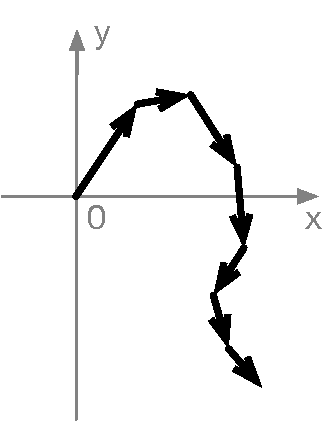
\includegraphics[width=0.2\linewidth]{reference_frame.pdf}
    \caption{Graphical explanation of the estimated positions of the robot over time. The starting position defines the center of the reference coordinate system.}
    \label{fig:reference_frame}
\end{figure}

Another relative localization approach is \emph{visual} odometry which tries to
fulfill the same goal as simple odometry but instead of motor or wheel
movements, it uses camera images. Classic approaches use techniques like optical
flow or feature matching between successive images in order to determine a
direction of movement between those two points in time.

The method we are going to present in this work is a visual odometry-based
approach but uses deep learning for determining the change of movement between
successive images. The original paper by Wang \etal{} \cite{wang2017deepvo} was
published in 2017 and describes the structure of a deep neural network
and evaluates its performance on the well-known KITTI dataset
which contains camera images and pose estimations of a car (a detailed
explanation is given in section~\ref{sec:deepvo:original}.

This paper is structured as follows. Section~\ref{sec:deepvo:original} presents
the idea and structure of the DeepVO Network and
Section~\ref{sec:deepvo:approach} gives a short explanation of how we
implemented it in TensorFlow. Section~\ref{sec:evaluation:data} will elaborate
on how we gathered data for training and testing. In
Section~\ref{sec:evaluation:results} we present the training behavior and
performance results of the our DeepVO implementation.


% --------------- %
% SECTION: DeepVO %
% --------------- %
\section{DeepVO Model}
\label{sec:deepvo}
In this section, the DeepVO network is presented (see Section~\ref{sec:deepvo:original}) together with our variant implemented in TensorFlow (see Section~\ref{sec:deepvo:approach}).


% -------------------------- %
% SUBSECTION: ORIGINAL PAPER %
% -------------------------- %
\subsection{Original Paper}
\label{sec:deepvo:original}

\begin{figure}[tbh]
    \centering
    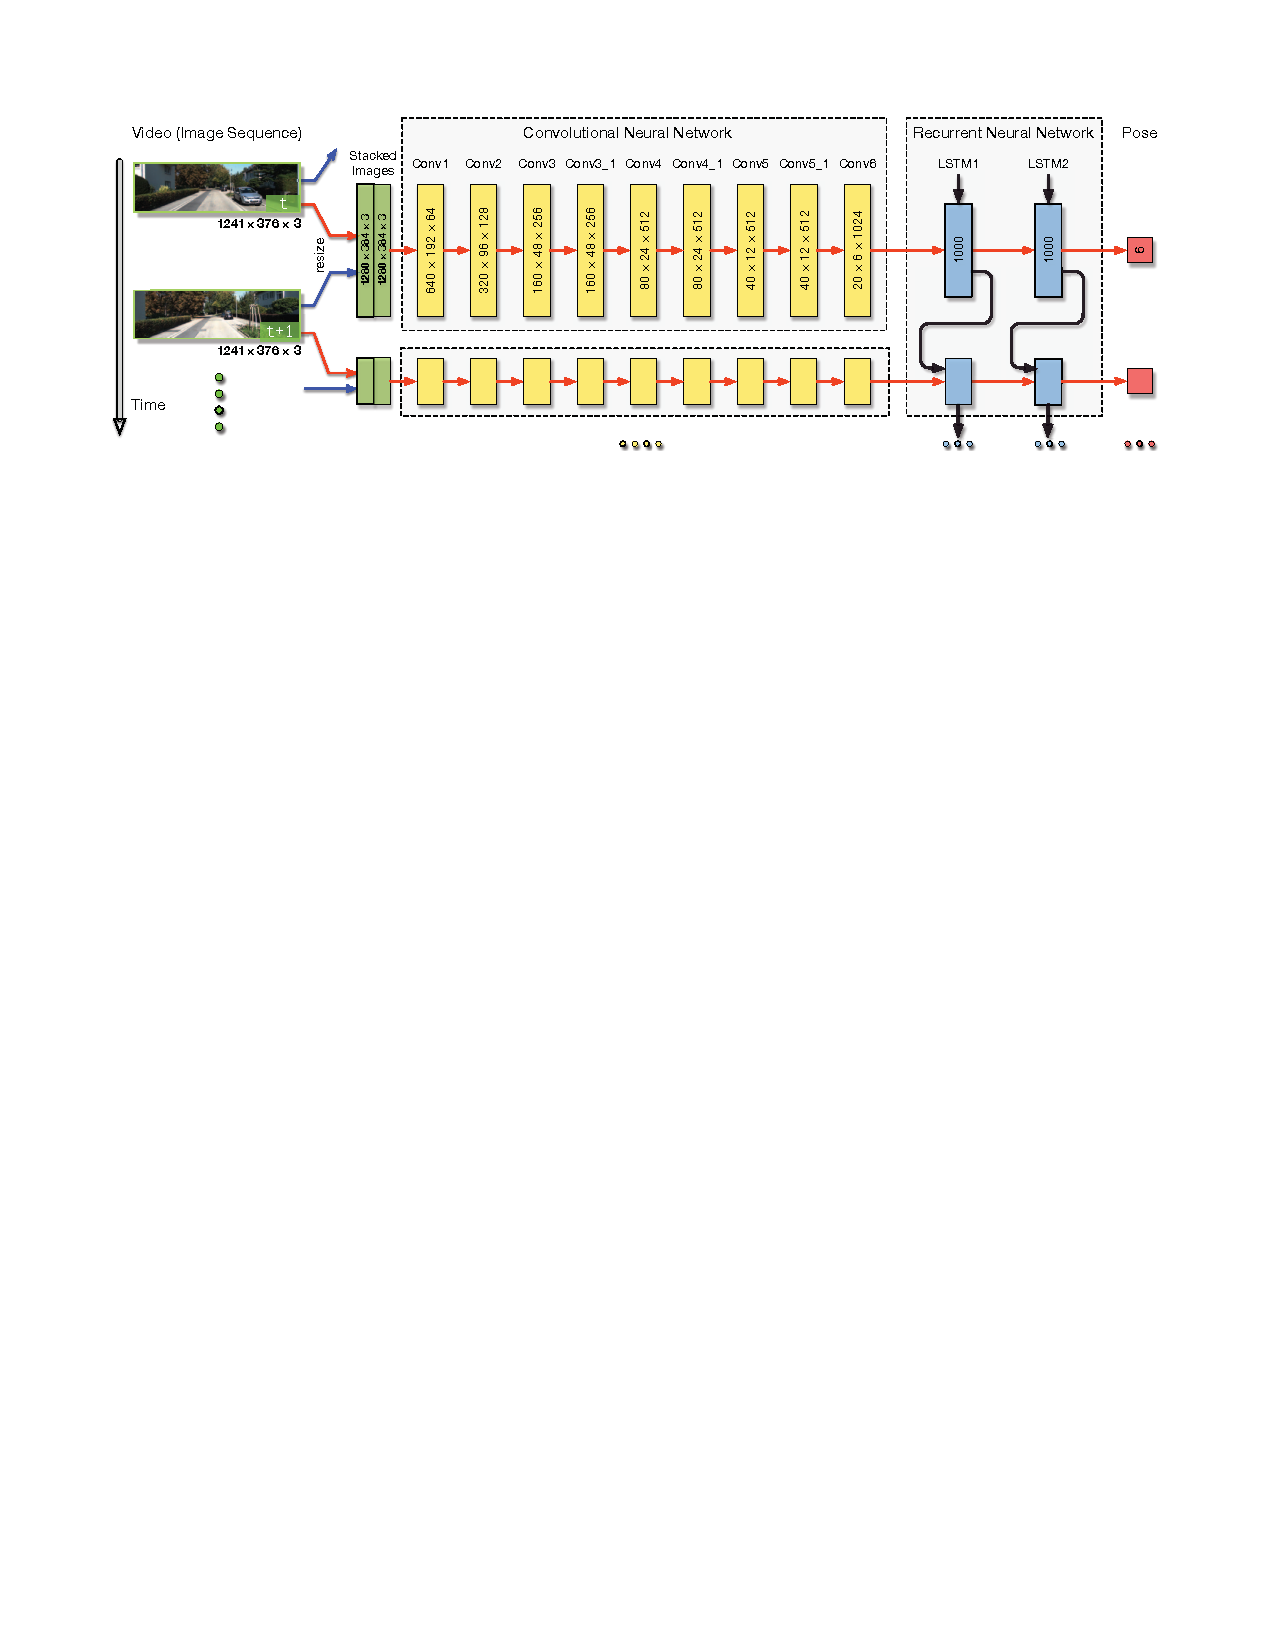
\includegraphics[width=\linewidth]{network.pdf}
    \caption{The structure of the network. Figure taken from \cite{wang2017deepvo}.}
    \label{fig:network}
\end{figure}

% TODO: Explain the deepVO model

The architecture for end-to-end learning of robot pose estimation is a recurrent
CNN where the convolutional portion is based on FlowNetSimple \cite{flownet} to
estimate the optical flow between successive images. The convolutional layers
are shown in \autoref{tab:cnn}
shows the network. Two successive images are stacked together and labeled with
the second image's pose. The stacked tensor is fed into the CNN to learn
features and estimate the optical flow. Subsequent LSTM layers are used to learn
consistent pose estimates from several timesteps in the past. The LSTM cells are
equipped with 1000 memory units.

\begin{table}
    \centering
    \caption{FlowNet CNN layers}
    \label{tab:cnn}
    \begin{tabular}{cccrc}
        Layer & kernel size & strides & filters & activation\\\hline
        1     & 7           & 2       & 64      & reLU\\
        2     & 5           & 2       & 128     & reLU\\
        3     & 5           & 2       & 256     & reLU\\
        4     & 3           & 1       & 256     & reLU\\
        5     & 3           & 2       & 512     & reLU\\
        6     & 3           & 1       & 512     & reLU\\
        7     & 3           & 2       & 512     & reLU\\
        8     & 3           & 1       & 512     & reLU\\
        9     & 3           & 2       & 1024    & -\\\hline
    \end{tabular}
\end{table}

Not mentioned in the paper, a dense sigmoid layer with 6 output units is added
to map the LSTM state onto three translation and rotation values.

The training loss is given as the mean squared error between network output and
target pose, summed over batch and time dimensions.
\begin{align}
    L(\text{Batch}; \theta) = \frac{1}{B} \sum^{B}_{i=1} \sum^{T}_{k=1}
    \Vert\hat{p}_{i,k} - p_{i,k} \Vert^2 + \kappa \Vert \hat{\phi}_{i,k} - \phi_{i,k} \Vert^2
\end{align}

where $\kappa$ is introduced as a weighting factor since translational and
rotational units are not directly comparable. \cite{wang2017deepvo} use the
Adagrad optimizer with a learning rate of 0.001. Futher parameters such as the
batch size, sequence length, dropout details, and dropout details are
missing from the paper.

A pretrained FlowNet model is used to speed up convergence.

% -------------------- %
% SUBSECTION: APPROACH %
% -------------------- %
\subsection{Our Approach}
\label{sec:deepvo:approach}
% TODO: Explain how we implemented the model described in the paper
% TODO: --> This includes other implementations we found on the web? or problems we had, or simply stuff we did'nt know better

Our implementation attempts to follow \cite{wang2017deepvo} and thus implements
all details from the paper, including loading FlowNet weights.
However, we were not able guess some hyperparameters
used for training. Hyperparameter optimization was also hampered by the fact
that it appears to be impossible to train this architecture with reasonable
layer sizes even on a powerful Tesla Volta GPU with 16GB of VRAM. Already on
small batch sizes ($\sim 10$) and sequence lengths ($\sim 10$), the network cannot be
trained even with a reduction of the LSTM state sizes. This observation calls
into question the claim that \cite{wang2017deepvo} trained the network on a
single K80 GPU.

While the paper makes no mention of treating angle differences in any particular
way in the loss function, we ensured the angular difference between estimate and
target rotation is always in the range $[-\pi,\pi]$. Without special
consideration, the difference between e.g. $1^\circ$ and $359^\circ$ would come out as
$358^\circ$ instead of $-2^\circ$. We thus compute the difference in the rotational
component as
\begin{align}
    \text{diff}(\hat{\phi}_i,\phi_i) = \atantwo\left(\sin\hat{\phi}_i - \phi_i,
    \cos{\hat{\phi}_i -\phi_i}\right)
\end{align}

This ensures the difference will have the proper sign and be in the interval
$[-\pi,\pi]$.

% -------------------- %
% SUBSECTION: SOFTWARE %
% -------------------- %
\subsection{Overview of the software}
\label{sec:deepvo:software}

Our code is written for for Python 3.6 against the 1.4 version of TensorFlow. A
conda environment specification is provided in \texttt{tfenv.txt} for
convenience. The code is heavily documented with Sphinx and the numpydoc plugin,
and documentation in various formats can be created by running \texttt{make} from the
\texttt{doc/} directory.

The purpose of the individual source files is as follows:
\begin{itemize}
    \item \texttt{main.py} -- Access to the training procedure
    \item \texttt{data\_manager.py} -- Data loading from disk
    \item \texttt{flownet.py} -- Global data for loading FlowNet weights
    \item \texttt{model.py} -- Definition of the main RCNN class
    \item \texttt{performance\_visualizer.py} -- Plotting functions for network performance
    \item \texttt{preprocess\_data.py} -- Preprocessing routines for data type
        conversion and mean-normalization
    \item \texttt{utils.py} -- Miscellaneous utilities.
\end{itemize}

More details are provided in the compiled documentation (simply open
\texttt{index.html}).

% ------------------- %
% SECTION: EVALUATION %
% ------------------- %
\section{Training \& Evaluation}
\label{sec:evaluation}
In this Section the data acquisition for training and testing is presented (see Section~\ref{sec:evaluation:data}), as well as the training progress and its performance results (see Section~\ref{sec:evaluation:results}).


% --------------------------- %
% SUBSECTION: DATA ACQUISTION %
% --------------------------- %
\subsection{Data Acquisition}
\label{sec:evaluation:data}
\begin{figure}[htb]
    \centering
    \begin{subfigure}[t]{0.6\linewidth}
            \centering
            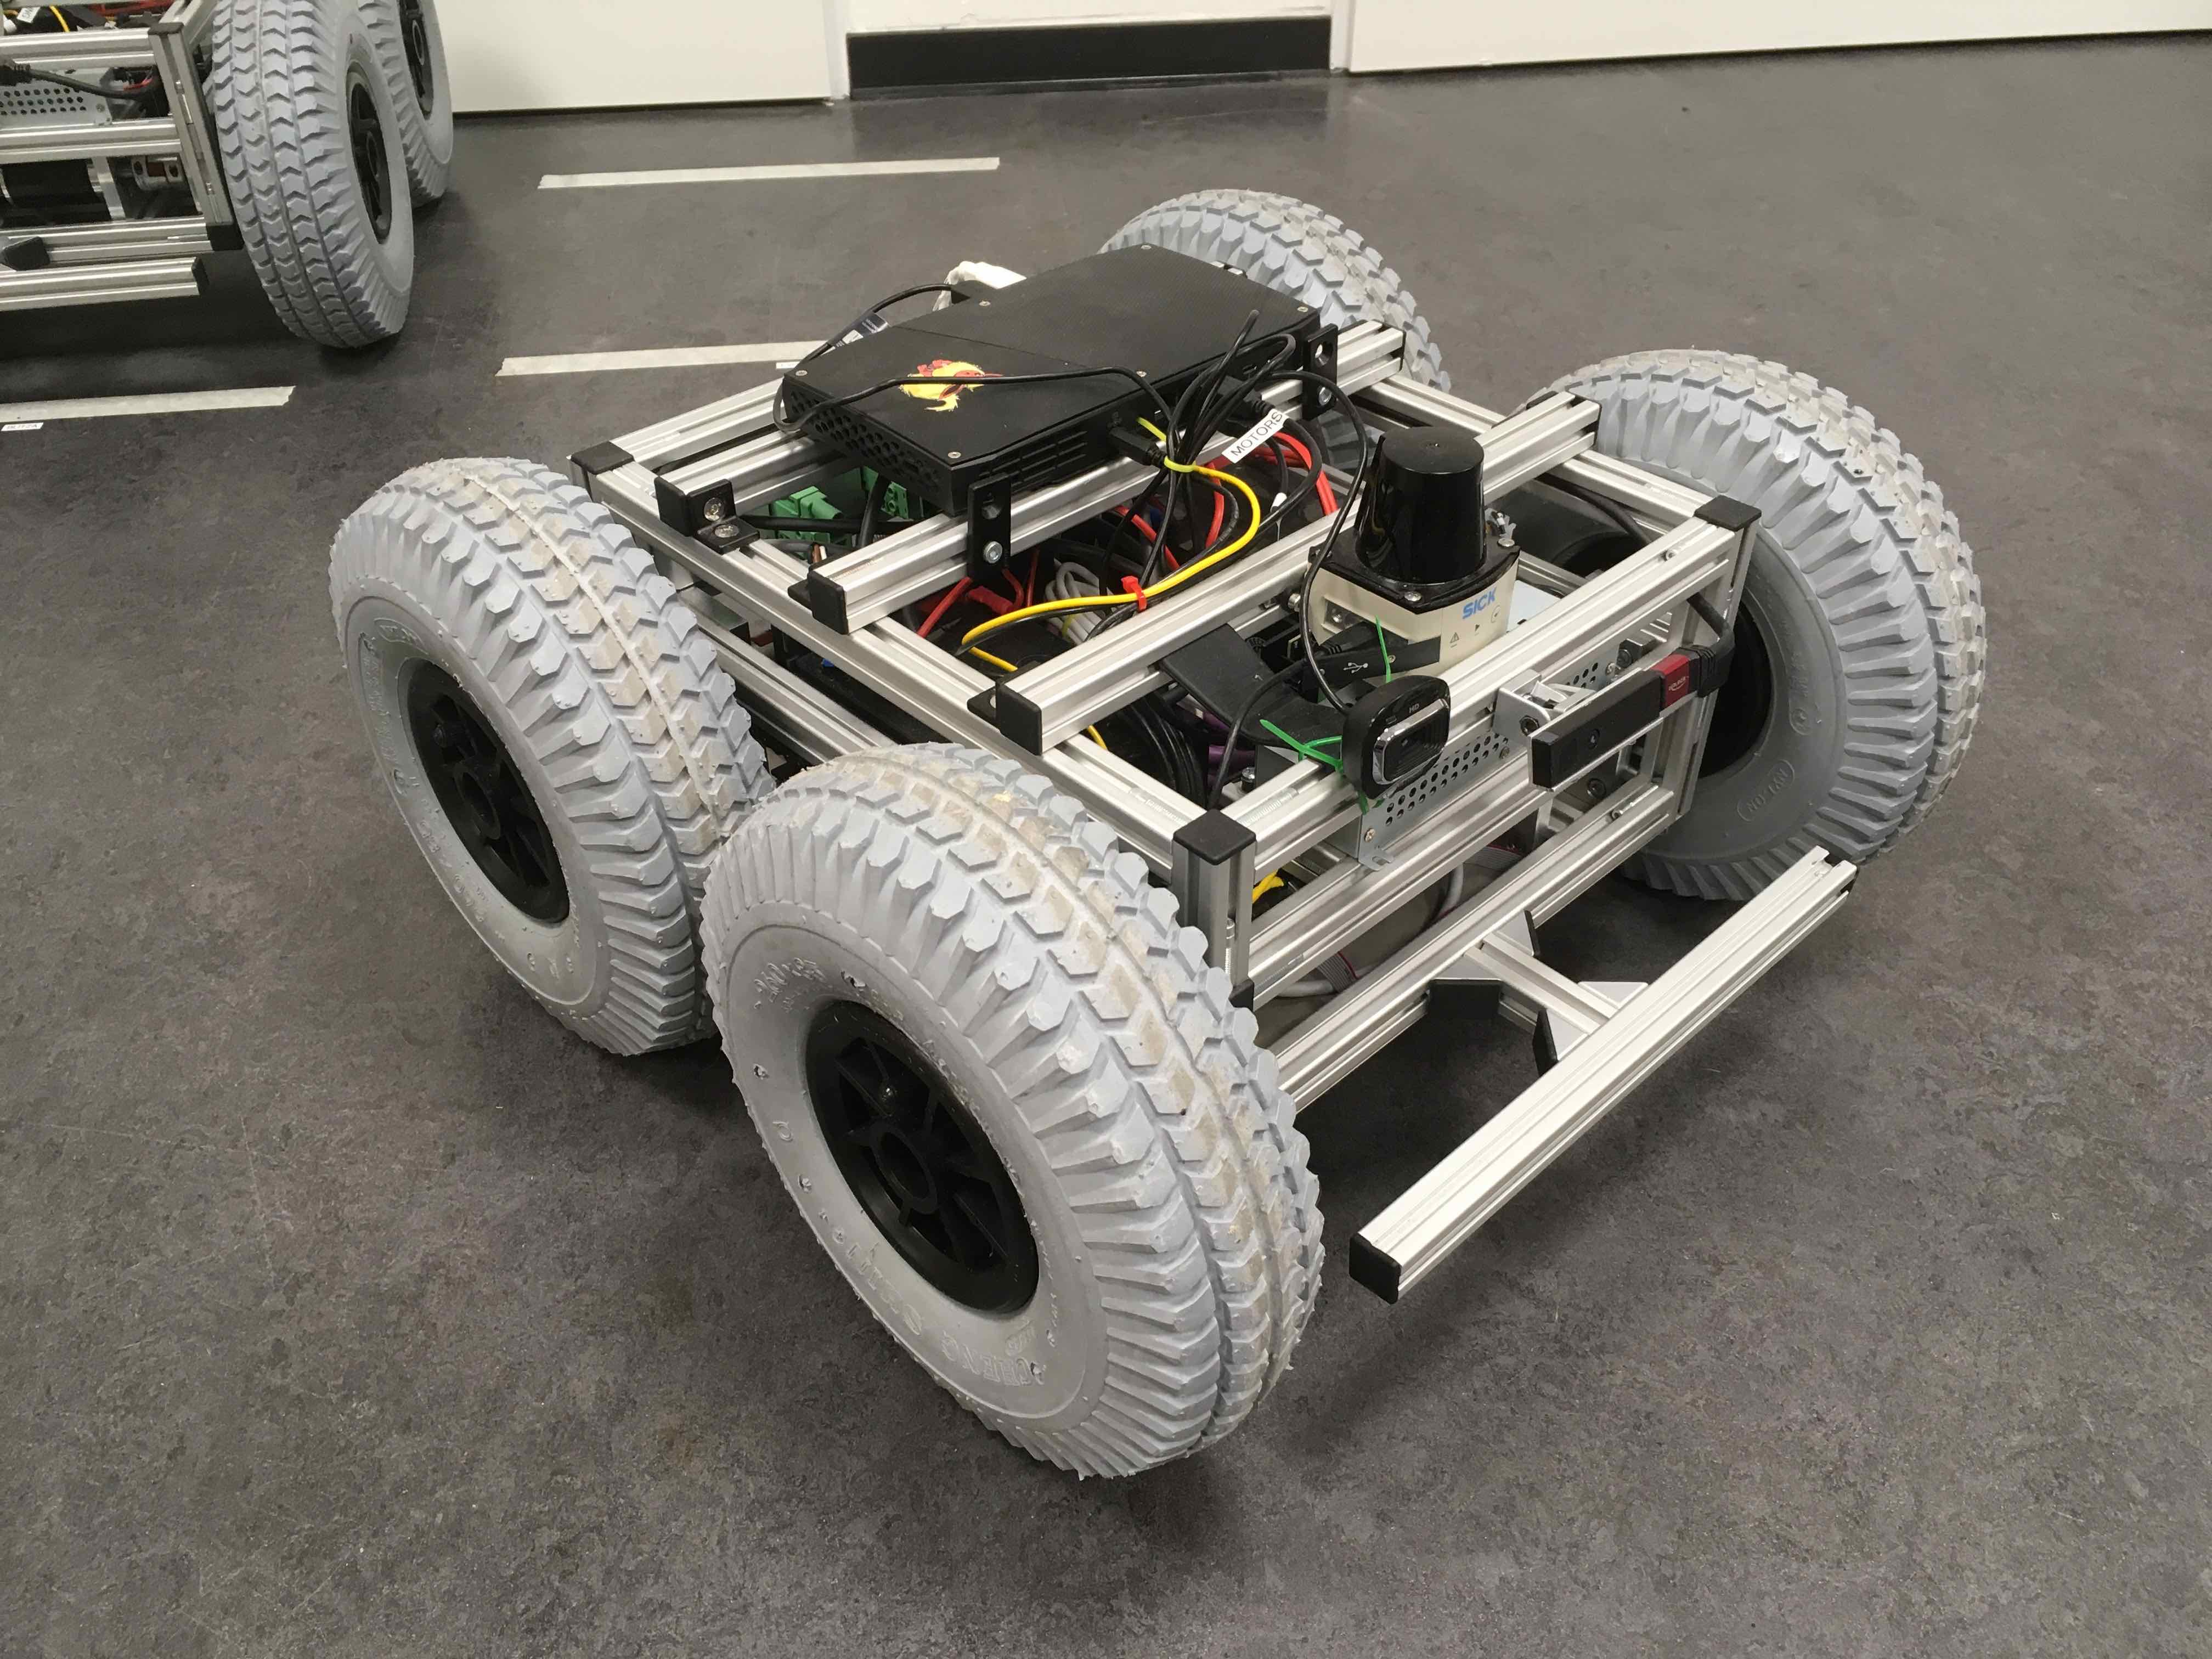
\includegraphics[width=0.9\linewidth]{robot_small.jpg}
            \caption[]{The ceres robot used for data acquisition.}
            \label{fig:robot}
    \end{subfigure}
    \begin{subfigure}[t]{0.39\linewidth}
            \centering
            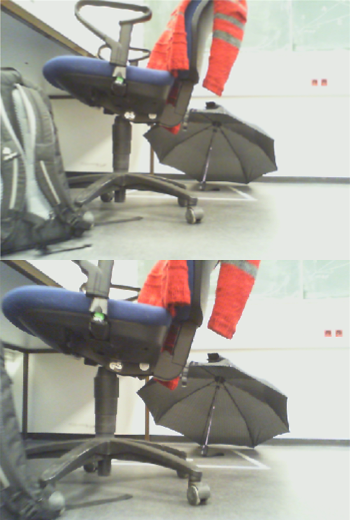
\includegraphics[width=0.75\linewidth]{image_pair.png}
            \caption[]{Exemplary successive images taken from the robots camera.}
            \label{fig:camera_images}
    \end{subfigure}
    \caption[]{Both figures depict the setup of our data acquisition.}
    \label{fig:setup}
\end{figure}

% TODO:
% - Das ist der Roboter
% - Eigene Daten aufnehmen
%   - ROSbags mit Images und poses
%       - ApproximateTimeSynchronizer
%
% - preprocessing
%   - float/mean images
%
% - Data Handling
%   - Sequences
%       - relative poses
%       - stacked images
%   - Shuffling
%   - test & training data batches

% --------------------------- %
% SUBSECTION: TRAINING        %
% --------------------------- %
\subsection{Training}
\label{sec:evaluation:training}

For training, we evaluated minimal parameters on a 1050Ti GTX card with 4GB of
VRAM, as well as a parallel computer with 56 Intel Xeon cpus (which turned out
to be useless), and, lastly, several AWS P2 and P3 instances, with Tesla K80 and
V100 cards, respectively. However, we were not able to obtain useful results in
the limited time available to us, since practical parameter combinations quickly
exceeded any GPU memory.


% ------------------- %
% SUBSECTION: RESULTS %
% ------------------- %
\subsection{Results}
\label{sec:evaluation:results}
<<<<<<< HEAD

Tba.

% ---------------------- %
% SUBSECTION: GREETINGS %
% ---------------------- %
\section{Room for Nonsense}
\label{sec:nonsense}
The authors would like to thank Thomes Wiemann for repeatedly failing to follow
through on his promise to secure an Nvidia hardware grant in order to obtain a
potent graphics card.


% --------------------- %
% SECTION: BIBLIOGRAPHY %
% --------------------- %
\newpage
\printbibliography


\end{document}
